\documentclass{article}
\usepackage{graphicx}
\usepackage{float}
\usepackage{titlesec}
\usepackage{datetime}
\usepackage{geometry}
\usepackage{placeins}
\usepackage{minted}
\usepackage{xcolor}
\usepackage{listings}
\usepackage{caption}
\usepackage[document]{ragged2e}
\usepackage[hidelinks]{hyperref}
\usepackage{fixltx2e}
\geometry{
 a4paper,
 left=25mm,
 top=25mm,
 }
\newdateformat{daymonthyear}{\THEDAY .\THEMONTH .\THEYEAR}
\title{
  \centering
  
\includegraphics[width=\textwidth]{images/logo_PWr_kolor_poziom.png}\\
  \fontsize{28pt}{30pt}\selectfont Sprawozdanie 2\\
  \fontsize{14pt}{30pt}\selectfont Ćwiczenie 4.Oświetlenie scen}
\author{Krzysztof Zalewa}
\date{\daymonthyear\today}
\renewcommand*\contentsname{Spis treści}
\renewcommand{\figurename}{Rysunek}
\renewcommand{\listingscaption}{Fragment kodu}
\begin{document}
  \maketitle
  \pagebreak
  \tableofcontents
  \section{Wstęp teoretyczny}
  \subsection{Model Phonga}
  Model Phonga lub oświetlenie Phonga to model lokalnego odbicia światła. By
  uzyskać najlepsze wyniki model ten uwzględnia trzy rodzaje światła (Rys1):
  \begin{itemize}
    \item \textbf{Światło kierunkowe(ang. Specular)} - refleksy odbite zgodnie z prawem Snella 
    \item \textbf{Światło rozproszone(ang. Diffuse)} - wpływ bezpośerednego oświetlenia
    \item \textbf{Światło otoczenia(ang. Ambient)} - jednorodne światło oświetlające cały obiekt
  \end{itemize}
  \begin{figure}[ht]
    \centering
    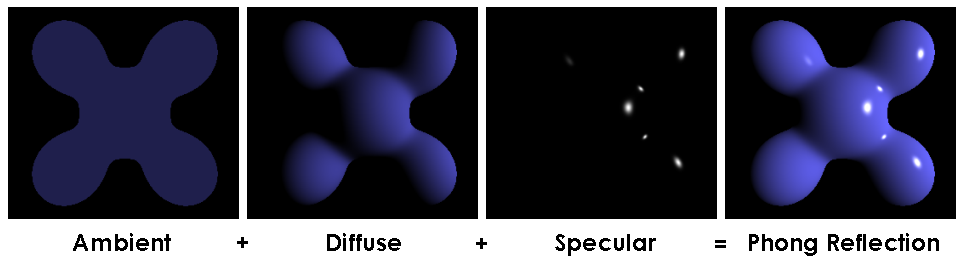
\includegraphics[width=\textwidth]{images/Phong_components_version_4.png}
    \caption{Model odbicia światła Phonga}
    \label{fig:phong}
  \end{figure}
  \FloatBarrier
  Każdy z materiałów na scenie ma zdefiniowane wartości $K_s,K_d,K_a$ 
  i alfa. Gdzie pierwsze trzy to stosunek odbicia światła (kolejno) kierunkowego,rozproszonego i otoczenia. 
  Alfa to z kolei połysk
  \subsection{Model Gourauda}
  Cieniowanie Gourauda to metoda interpolacj polegająca na oświetlaniu wierzchołków 
  w siatkach trójkątów i interpolacji wyników na cały trójkąt. Cieniowanie Gourauda
  jest uznawane za lepsze od cieniowania płaskiego i wymaga znacznie mniej obliczneń
  niż cieniowanie Phonga ale daje gorsze wyniki.
  \begin{figure}[ht]
    \centering
    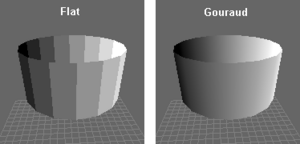
\includegraphics[width=\textwidth]{images/D3D_Shading_Modes.png}
    \caption{Model cieniowania Gourauda}
    \label{fig:gour}
  \end{figure}
  \FloatBarrier
  \subsection{Wektor normalny}
  Wektor normalny to wektor prostopadły do płaszczyzny stycznej do danej powierzchni w danym punkcie.
  Pozwala to na rozróżnienie "Przodu" i "Tyłu" powirzchni co z kolei pozwala na ukrycie niewidocznych 
  powierzchni (funkcja glCullFace)
  \begin{figure}[ht]
    \centering
    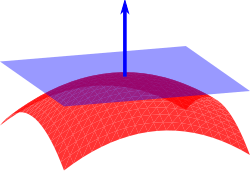
\includegraphics[width=\textwidth]{images/Surface_normal_illustration.svg.png}
    \caption{Model cieniowania Gourauda}
    \label{fig:normal}
  \end{figure}
  \FloatBarrier
  \section{Zadanie laboratoryjne}
  \subsection{Treść zadania}
  W ramach zadania należało do poprzednio stworzonego programu dodać dwa źródła 
  światła. W kolorach przeciwstawnych (Czerwone i zielone). Światła te powinny 
  świecić w stożku.
  \subsection{Opis działania programu}
  \raggedright
  Zgodnie z treścią zadania program rysuje 4 obiekty. Domyślnie 
  jajko i czajnik rysowane są w kolorze białym. Jednakże jest 
  możliwość zmiany koloru na losowy. Wyświetlone obiekty można 
  obracać za pomocą myszki (Przycisk musi być wciśnięty i 
  przytrzymany). Program implementuje dwa światła niebieskie i czerwone.\linebreak 
  \textbf{Kontrola obrotu:}\linebreak  
  \textbf{F1} - tryb obrotu obiektu\linebreak
	\textbf{F2} - tryb obrotu kamery\linebreak
	\textbf{F3} - tryb obrotu swiatlem 1 (Czerwone)\linebreak
	\textbf{F4} - tryb obrotu swiatlem 2 (Zielone)\linebreak
  \textbf{ESC} - Powrót do menu (okno konsolowe)\linebreak 
  \textbf{Ruch myszy w osi X} - Obrót kamery w osi X\linebreak 
  \textbf{Ruch myszy w osi Y} - Obrót kamery w osi Y\linebreak 
  \textbf{Scroll up} - Przybiliżenie obiektu\linebreak 
  \textbf{Scroll down} - Oddalenie obiektu\linebreak 
  \subsection{Kod programu}
  \begin{frame}
    \scriptsize
    \inputminted[
        style={vs},
        breaklines,
        breakanywhere, 
        linenos, 
        tabsize=4 
    ]{c++}{Lab4.cpp}
    \vspace{1em}
    \captionsetup{justification=centering}
    \captionof{listing}{Fragment kodu z programu}
    \label{lst:code}
  \end{frame}
  \begin{frame}
    \scriptsize
    \inputminted[
        style={vs},
        breaklines,
        breakanywhere, 
        linenos, 
        tabsize=4 
    ]{c++}{Egg.cpp}
    \vspace{1em}
    \captionsetup{justification=centering}
    \captionof{listing}{Kod Egg.cpp}
    \label{lst:egg}
  \end{frame}  
  \begin{frame}
    \scriptsize
    \inputminted[
        style={vs},
        breaklines,
        breakanywhere, 
        linenos, 
        tabsize=4 
    ]{c++}{Light.cpp}
    \vspace{1em}
    \captionsetup{justification=centering}
    \captionof{listing}{Kod Light.cpp}
    \label{lst:light}
  \end{frame}
  \section{Wnioski}
  Na zajęciach nie udało się ukończyć programu. Po pracy w domu program działa poprawnie.
  \section{Źródła}
  \begin{itemize}
    \item \url{https://gniewkowski.wroclaw.pl/gk/lab5.pdf}
    \item \url{https://en.wikipedia.org/wiki/Phong_reflection_model}
    \item \url{https://en.wikipedia.org/wiki/Gouraud_shading}
    \item \url{https://pl.wikipedia.org/wiki/Wektor_normalny}
  \end{itemize}
\end{document}